\section{Cutting LLVM Functions}
\label{sec:cut}

Using a typical function in LLVM IR as the specification, it is not
practical to directly synthesize an optimized version of that
function.
%
The state of the art in program synthesis simply does not scale up to
the size of LLVM functions found in the wild.
%
Instead, \minotaur{} takes a divide-and-conquer approach: we individually
attempt to optimize each instruction in an LLVM function by extracting
a \textit{cut}---a subset of that instruction's dependencies.
%
If this cut of LLVM instructions can be optimized by program synthesis
then, by the compositionality of refinement, so can the original LLVM
function.
%
The rest of this section describes this process in more detail.


\subsection{Problem Statement}

Given a function $F$, an instruction $I$ within $F$, and a depth
bound $B$, our goal is to create a new LLVM function $C$ that:
%
\begin{enumerate}
\item
  is loop-free,
\item
  returns the value computed by $I$, and
\item
  contains every instruction in $F$ that can be reached by following
  up to $B$ backwards data, control, and memory dependency edges.
\end{enumerate}
%
Informally, we can think of $C$ as summarizing a subcomputation in
$F$, that is (hopefully) tractable for an SMT solver to reason about.


When an instruction is part of $C$ but its inputs are not, then these
become free inputs---these are implemented by adding them as
parameters to $C$.
%
We can think of every instruction that is not part of the cut as being
part of a residual function $R$.
%
However, note that \minotaur{} does not explicitly construct $R$---it
computes and optimizes $C$, and then applies the discovered
optimization, if any, directly to $F$ using a rewrite mechanism
described in Section~\ref{sec:rewrite}.


\subsection{Example}

\begin{figure}
  \centering
  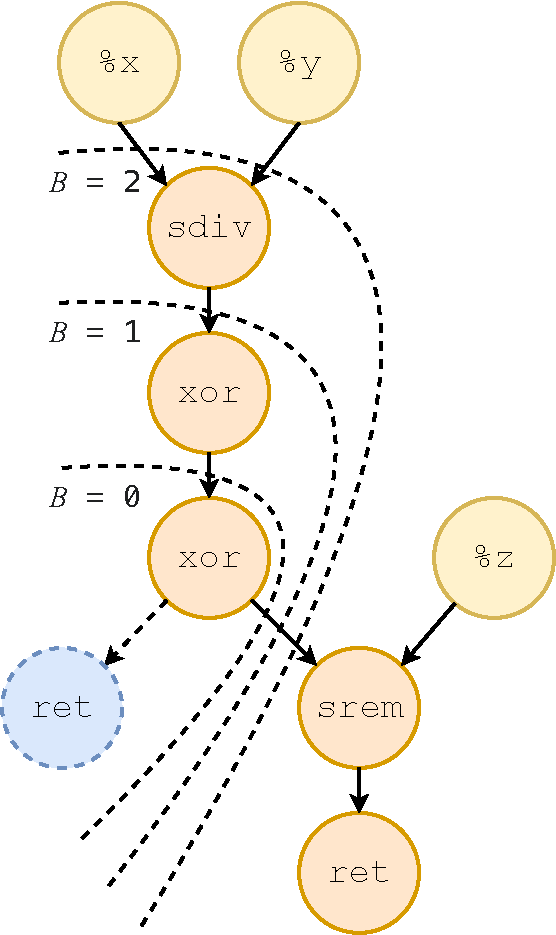
\includegraphics[width=0.5\linewidth]{figures/cut-depth.pdf}
  \caption{Example of cutting an LLVM function}
  \label{fig:cut-depth}
\end{figure}

Consider this LLVM function that takes three 64-bit arguments and
returns a 64-bit value, where \texttt{sdiv} is signed integer division
and \texttt{srem} is the signed integer modulus operator:

%%% https://gcc.godbolt.org/z/Wes9sPKGW

{\begin{quote}
\begin{verbatim}
define i64 @f(i64 %x, i64 %y, i64 %z) {
  %a = sdiv i64 %x, %y
  %b = xor i64 %a, -1
  %c = xor i64 %b, -1
  %d = srem i64 %c, %z
  ret i64 %d
}
\end{verbatim}
\end{quote}}

Figure~\ref{fig:cut-depth} illustrates various cuts of this function.
%
If we cut this function with respect to \texttt{\%c} with $B = 0$ then
we get the following decomposition (however, again, please bear in
mind that \minotaur{} does not actually construct $R$---we show it here to
make the explanation concrete):

\begin{multicols}{2}
{\begin{quote}
\begin{verbatim}
define i64 @r0(i64 %x, i64 %y, i64 %z) {
  %m = sdiv i64 %x, %y
  %n = xor i64 %m, -1
  %o = call i64 %c0(i64 %n)
  %p = srem i64 %o, %z
  ret i64 %p
}
\end{verbatim}
\end{quote}}
\columnbreak
{\begin{quote}
\begin{verbatim}
define i64 @c0(i64 %t1) {
  %t2 = xor i64 %t1, -1
  ret i64 %t2
}
\end{verbatim}
\end{quote}}
\end{multicols}

This is not useful, the cut \texttt{c0} contains too little context
to support any optimizations.
%
If we cut \texttt{f} with respect to \texttt{\%c} with $B = 1$ then we get:

\begin{multicols}{2}
{\begin{quote}
\begin{verbatim}
define i64 @r1(i64 %x, i64 %y, i64 %z) {
  %m = sdiv i64 %x, %y
  %o = call i64 @c1(i64 %m)
  %p = srem i64 %o, %z
  ret i64 %p
}
\end{verbatim}
\end{quote}}
\columnbreak
{\begin{quote}
\begin{verbatim}
define i64 @c1(i64 %t1) {
  %t2 = xor i64 %t1, -1
  %t3 = xor i64 %t2, -1
  ret i64 %t3
}
\end{verbatim}
\end{quote}}
\end{multicols}

This decomposition is useful: \texttt{c1} can be optimized to simply
return its argument.
%
If we increase the depth bound to two, then we would get:

\begin{multicols}{2}
{\begin{quote}
\begin{verbatim}
define i64 @r2(i64 %x, i64 %y, i64 %z) {
  %o = call i64 @c2(i64 %x, i64 %y)
  %p = srem i64 %o, %z
  ret i64 %p
}
\end{verbatim}
\end{quote}}
\columnbreak
{\begin{quote}
\begin{verbatim}
define i64 @c2(i64 %t1, i64 %t2) {
  %t3 = sdiv i64 %t1, %t2
  %t4 = xor i64 %t3, -1
  %t5 = xor i64 %t4, -1
  ret i64 %t5
}
\end{verbatim}
\end{quote}}
\end{multicols}

Here the cut \texttt{c2} can again be optimized (it can just return
\texttt{\%t3}), but now the solver must reason about a 64-bit signed
division---operations like this are difficult and frequently lead to
timeouts.
%
Choosing an appropriate depth bound is an empirical problem that
we address in Section~\ref{sec:loops}.


\subsection{Correctness Argument}

The composition of $R$ and $C$ is equivalent to the original function:
$F = R \circ C$.
%
In other words, the decomposition of $F$ into $R$ and $C$ preserves
the behavior of the original function---the difference is simply that
some dependency edges that were previously internal to $F$ now cross
the boundary between $R$ and $C$.


Next, if \minotaur{} can synthesize $C'$, an optimized function that
refines $C$, then we can compose that with the residual function to
get a new function $F' = R \circ C'$.
%
Since refinement is compositional, it follows that $F'$ refines $F$,
which is the property that we need for \minotaur{} to be a correct
optimizer.
%
The details of establishing a refinement relation between functions in
LLVM IR were presented by Lopes et al.~\cite{alive2}.


Alive2 is intended to be a sound refinement checker for LLVM
IR for LLVM functions that do not contain loops.
%
We avoid this potential unsoundness by ensuring that $C$ is loop-free,
in which case $C'$ is also loop-free since \minotaur{} never synthesizes a
loop.



\begin{algorithm}[tbp]
  %
\caption{Cut Extraction Algorithm}
  \begin{algorithmic}[1]
  \Function{ExtractCut}{\emph{F}: Function, \emph{I}: Instruction, \emph{B}: $\mathbb{N}$}
  \If{$I$ is in a loop}
    \State {\emph{AllowedBasicBlocks} $\gets $ all basic blocks in \emph{I}'s loop (innermost loop if nested)}
  \Else
    \State {\emph{AllowedBasicBlocks} $\gets$ all basic blocks in \emph{F} that is not in a loop}
  \EndIf
  \State {\emph{Harvested} $\gets \emptyset $}
  \State {\emph{Unknown} $\gets \emptyset $}
  \State {\emph{Visited} $\gets \emptyset $}
  \State {\emph{WorkList} $\gets$ \{ (\emph{I}, 0) \}}
  \While{\emph{WorkList} is not empty}
  \Comment{stage 1, instruction extraction}
  \State {(\emph{WI}, \emph{Depth}) $\gets $ \emph{WorkList}.pop()}
  \If {\emph{WI} $\in$ \emph{Visited}}
  \State \textbf{continue}
  \EndIf
  \State {Insert \emph{WI} into \emph{Visited}}
  \If{\emph{Depth} $>$ \emph{B}}
  \State {Insert \emph{WI} into \emph{Unknown}}
  \State {\textbf{continue}}
  \EndIf
  \If{\emph{WI} is not supported}
  \State {Insert \emph{WI} into \emph{Unknown}}
  \State {\textbf{continue}}
  \EndIf
  \State {\emph{BB} $\gets$ \emph{WI}'s basic block}
  \If{\emph{BB} $\notin$ \emph{AllowedBasicBlocks}} %$L$ $\land$ WI is not in $I$'s innermost loop}
  \State {Insert \emph{WI} into \emph{Unknown}}
  \State {\textbf{continue}}
  \EndIf
  \State {Insert \emph{WI} into \emph{Harvested}}
  \If{\emph{WI} is a Load instruction}
    \State {\emph{M} $\gets$ \emph{WI}'s linked \texttt{MemoryPhi} or \texttt{MemoryDef}}
    \If {\emph{M} is a \texttt{MemoryDef} $\wedge$ \emph{M} is a store}
    \State {\emph{MI} $\gets$ \emph{M}'s stored value}
    \State {Push (\emph{MI}, \emph{Depth} + 1) into \emph{WorkList} }
  \EndIf

  \Else
    \ForAll{operand \emph{Op} in \emph{WI}}
    \State {Push (\emph{Op}, \emph{Depth} + 1) into \emph{WorkList} }

    \EndFor
  \EndIf

  \State {\emph{T} $ \gets$ terminator of \emph{WI}'s basic block}
    \If {\emph{T} is a conditional branch instruction}
    \State {\emph{TI} $\gets$ \emph{T}'s condition value}
    \State {Push (\emph{TI}, \emph{Depth} + 1) into \emph{WorkList} }
    \EndIf

  \EndWhile
  \State {Insert every terminator instruction in \emph{F} to \emph{Harvested}}
  \State {Clone \emph{F} into \emph{C}}
  \Comment{stage 2, construct a loop-free LLVM function}
  \State {Delete instructions in \emph{C} except those in \emph{Harvested}}
  \State {Delete all back-edges in \emph{C}}
  \State {Add values in \emph{Unknown} to \emph{C} as function arguments}
  \State {Create return instruction for \emph{I} in \emph{C}}
  \State {\textbf{return} \emph{C}}
  \EndFunction
  \end{algorithmic}
  \label{alg:slicing}
\end{algorithm}


\subsection{Detailed Solution}

Algorithm~\ref{alg:slicing} shows the procedure that \minotaur{} uses to
extract a cut.
%
It works in two stages.
%
In the first stage, \minotaur{} determines which instructions will be part
of the cut, using a depth-bounded depth-first search.
%
During the search, two sets, \emph{Harvest} and \emph{Unknown}, are
propagated which will be used in the second stage for constructing the
cut.
%
\minotaur{} uses LLVM's LoopInfo pass~\cite{loopinfo} to identify loops in the
source function.
%
If instruction $I$ is in a loop, \minotaur{} will only extract
instructions that are defined inside the loop.
If the loop is nested, \minotaur{} will only extract instructions that are
defined inside the innermost loop.
\minotaur{} will give up if the loop is irregular.
%
If $I$ is not in a loop, \minotaur{} will skip the instructions that are in a loop.
%
\minotaur{} marks non-intrinsic function calls, operations on global
variables, and operations that are not recognized by Alive2 as
unsupported.
%
All unsupported operations, operations that are beyond the depth
limit, and operations that are outside the loop are discarded and
replaced with free inputs.


For each conditional branch instruction, \minotaur{} extracts the branch
condition, since these carry control flow information that is useful
during synthesis.
%
Similarly, when it extracts a load from memory, \minotaur{} consults
LLVM's MemorySSA pass~\cite{MemorySSA} to get a list of stores that
potentially influence the loaded value.
%
MemorySSA marks memory operations with one of the three memory access tags:
\texttt{MemoryDef}, \texttt{MemoryUse}, and \texttt{MemoryPhi}.
Each memory operation is associated with a version of memory state.
%
A \texttt{MemoryDef} can be a store, a memory fence, or any operation
that creates a new version of the memory state.
%
A \texttt{MemoryPhi} combines multiple \texttt{MemoryDef}s when
control flow edges merge.
%
A \texttt{MemoryUse} is a memory instruction that does not modify
memory, it only reads the memory state created by \texttt{MemoryDef}
or \texttt{MemoryPhi}; a load instruction is always a
\texttt{MemoryUse}.
%
Because it must overapproximate, \minotaur{} is conservative when finding
the load-affecting store: it starts from the loads
\texttt{MemoryUse}'s memory version and walks along the MemorySSA's
def-use chain,
%
and when the associated memory operation is a \texttt{MemoryDef}, it
checks if the operation is a store and pushes the stored value into
the worklist.
%
\minotaur{} gives up when the associated memory version is tagged with
\texttt{MemoryPhi}, or when the version is tagged with
\texttt{MemoryDef} but the operation is not a store instruction.


In the second stage, \minotaur{} builds the extracted function; it does
this by cloning the original function and then deleting all
instructions that are not in the cut.
%
\minotaur{} then deletes all the loop backedges so that the extracted
function is loop-free.
%
Finally, a return instruction is added to return the value computed by
the instruction that is the basis for the cut.

\begin{figure}
  \centering
  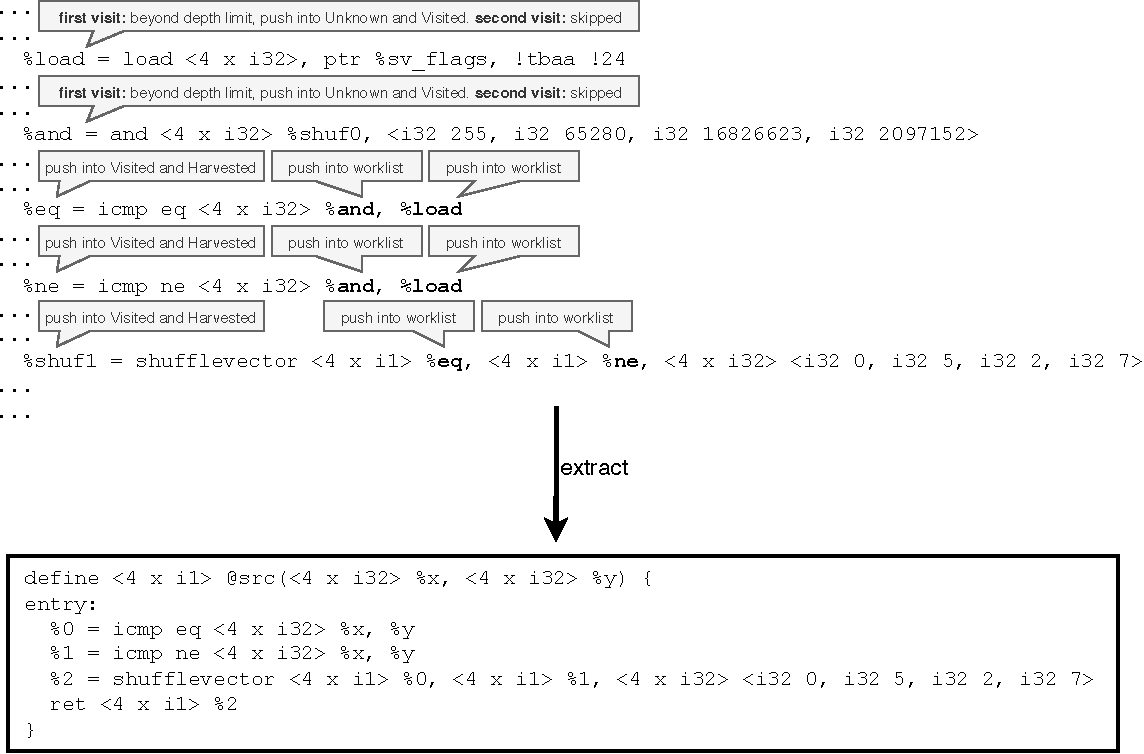
\includegraphics[width=\linewidth]{figures/slice.pdf}
  \caption{Example of cut extraction}
  \label{fig:cut}
\end{figure}


Figure~\ref{fig:cut} shows an example of cut extraction
for value \texttt{\%shuf1}.
%
The cutting algorithm starts on \texttt{\%shuf1} and walks along the
def-use chain to extract the instructions that are involved in the
computation of \texttt{\%shuf1}.
%
A new function is created to hold the extracted instructions shown
in the bottom of the figure.



\subsection{Relation to Previous Cut-Based Superoptimizers}

\minotaur's cut extraction algorithm is fundamentally more aggressive
than Bansal and Aiken's approach~\cite{Bansal06}, which extracted a
small window of sequential instructions.
%
It is also considerably more aggressive than Souper~\cite{souper},
which had a very limited view of control flow and refused to consider
memory operations, vector operations, and floating-point operations.